% CAPÍTULO 2: FUNDAMENTAÇÃO TEÓRICA
%   DEVE SER UM CAPÍTULO ENXUTO (LEAN)
%1. Elabore um parágrafo que introduz o capítulo: Este capítulo apresenta (descreva o objetivo do capítulo...). É constituído de N seções a saber...
%2. Desenvolvimento do capítulo: os conteúdos devem ser somente os necessários para o leitor entender a sua contribuição.
%3. Trabalhos relacionados: a última seção do Capítulo 2 deve apresentar o posicionamento da sua contribuição em relação à literatura. É um detalhamento da Justificativa apresentada na Introdução.
%4. Elabore um parágrafo que conclui o capítulo e introduz o capítulo seguinte.

This work use concepts from Human Factors and Co-design and is supported by tools such as Extended Reality (XR), more precisely VR, and some specific assessment methods using task performance, physiological measures and subjective measures. This chapter introduces the need-to-know of each of these to help to better understand this Master's thesis. Each subject is introduced in the following 5 sections

\section{Human Factor or Ergonomics}
\label{sec:human_factors}

    Studies started during the Second World War because of the performance shortfalls and failures noted in manned equipment. These studies showed that these problems could diminish when engineering, psychology and physiology were gathered when designing a system that was to be handled by a human being \cite{sandom2004human}.

This area of study was named "Human Factors" in the United States and "Ergonomics" in Europe. Despite this difference in the names, today they are considered the same field of study. The International Ergonomics Association (IEA) defines Human Factors, and Ergonomics, as the following:

\begin{quote}
    Ergonomics (or human factors) is the scientific discipline concerned with the understanding of interactions among humans and other elements of a system, and the profession that applies theory, principles, data and methods to design in order to optimize human well-being and overall system performance. Human Factors professionals contribute to the design and evaluation of tasks, jobs, products, environments and systems in order to make them compatible with the needs, abilities and limitations of people \cite{karwowski2012discipline}.
\end{quote}

Besides being synonyms, this definition shows that humans are a variable inside a system and their interactions should be studied and that is the focus of Human Factors \cite{sandom2004human, sanders1998human, dul2003ergonomics}. 

Humans handle devices, machines and equipment during their daily activities and all of these manipulations are susceptible to accidents or failures that can happen because of the interaction between operator, equipment and environment. Each interface with the operator can be a factor, for example:

\begin{itemize}
    \item The operator's body position during an activity;
    
    The position can impact the comfort felled by the operator and this impacts its concentration throughout the activity, therefore, impacting the success rate or the chance of some accident happening \cite{sanders1998human}.
    
    \item The environment's lighting;
    
    The illumination can make details easier to be noted without provoking discomfort or distraction to the user and even increase productivity \cite{sanders1998human}.
    
    \item The information displayed and manipulation of the device.
    
    The way information is displayed on a screen, figure or text impacts how efficiently it will be understood by the operator. If this takes too long it can draw the operator's attention for too long and compromise his/her reaction time.
    
\end{itemize}

Taking humans into account when designing a product or a system is one of the principles for human factors \cite{sandom2004human} and the results of this human-centred design are already an ISO Standard (BS EN ISO 13407 "Human-centred design processes for interactive systems"). This standard was originally written for computer-based-systems, but is easily applicable in other scenarios and areas \cite{sandom2004human}.

It is important to say that when it is said "User", it doesn't mean that one needs to design a product specifically for an individual. The design has to be suited to everyone \cite{dul2003ergonomics}.

"Human-Machine systems" (on this thesis, for now on, called simply "Systems"), are interactions between humans and machines. These systems are designed to have an input, or demand, and an output, or product. Here, "machine" can be any manipulated object, from a simple screwdriver to a car, or some machine operated by more than one human, like a cargo ship for example. The Figure \ref{fig:human_machine_representaion} represent a general human-system machine interaction.

\begin{figure}[!htb]
    \centering

    \tikzstyle{arrow} = [rounded corners, line width = 1mm, bend left = 15, ->]
    
    \resizebox{0.85\width}{!}{
    \begin{tikzpicture}[node distance=1cm]
        
        \node (information) {
\includegraphics[width=.15\textwidth]{Fundamentação/Fatores Humanos/thinking.png}} 
        node(t_information)[below of = information,yshift=-0.75cm] {Information}
        node(t_information2)[below of = t_information,yshift=0.25cm] {processing};
        
        \node (controlling) [right of=information, xshift=5cm, yshift=-3cm] {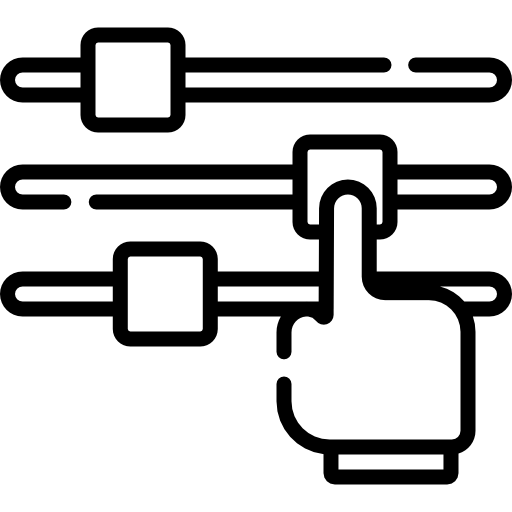
\includegraphics[width=.15\textwidth]{Fundamentação/Fatores Humanos/slider.png}}
        node(t_controlling)[below of = controlling,yshift = -0.75cm] {Controlling};
        
        \node (controls) [below of=controlling, yshift=-5cm,] {
\includegraphics[width=.15\textwidth,angle=90,origin=c]{Fundamentação/Fatores Humanos/control.png}} 
        node(t_controls) [below of = controls, yshift = -0.75cm]{Controls};
        
        \node (machine) [left of=controls, xshift=-5cm, yshift=-2cm] {
\includegraphics[width=.15\textwidth]{Fundamentação/Fatores Humanos/machine.png}} 
        node(t_machine) [below of = machine, yshift = -0.75cm]{Operation};
        
        \node (display) [left of=machine, xshift=-5cm, yshift=2cm] {
\includegraphics[width=.15\textwidth]{Fundamentação/Fatores Humanos/monitor.png}} 
        node(t_display) [below of = display, yshift = -0.75cm]{Display};
        
        \node (senses) [left of=information, xshift=-5cm, yshift=-2cm,] {\begin{tikzpicture}[node distance=1cm]
    \centering
    
    \node (eye) {
\includegraphics[width=.075\textwidth]{Fundamentação/Fatores Humanos/eye.png}};
    
    \node (ear) [right of=eye, yshift=-0.65cm] {
\includegraphics[width=.075\textwidth]{Fundamentação/Fatores Humanos/ear.png}};
    
    \node (nose) [left of=ear, yshift=-0.65cm] {
\includegraphics[width=.075\textwidth]{Fundamentação/Fatores Humanos/nose.png}};
    
    \node (hand) [right of=nose, yshift=-0.85cm] {
\includegraphics[width=.075\textwidth]{Fundamentação/Fatores Humanos/hand.png}};

\end{tikzpicture}} 
        node(t_senses) [below of = senses, yshift = -1.25cm]{Senses};
        
        \node (human) [below of=information, yshift=-4.75cm] {\Large{Human}};
        \node (human) [above of=machine, yshift=3.25cm] {\Large{Machine}};
        \node (human) [above of=information, yshift=1cm] {\Large{Work Environment}};
        
        \node (left_point) [left of=display, xshift=-2, yshift=2.75cm] {};
        \node (right_point) [right of=left_point, xshift=14cm] {};
        
        \node (input) [left of=machine, xshift=-5cm, yshift=-2cm] {\Large{Input}};
        \node (output) [right of=machine, xshift=5cm, yshift=-2cm] {\Large{Output}};
        
    
        \draw [arrow] (information.east) to (controlling.north west);
        \draw [arrow] (t_controlling.south) to (controls.north);
        \draw [arrow] (controls.west) to (machine.east);
        \draw [arrow] (machine.west) to (display.east);
        \draw [arrow] (display.north) to (t_senses.south);
        \draw [arrow] (senses.east) to (information.west);
        \draw [arrow] (input.east) -- (machine);
        \draw [arrow] (machine) -- (output.west);
        \draw [dashed,gray] (left_point) to (right_point);
        
        \draw (-8,-14) rectangle(8cm,1.5cm);
        
    \end{tikzpicture}
    }
    \caption{Human-Machine system representation \cite{sanders1998human}.}
    \label{fig:human_machine_representaion}
\end{figure}

\section{Mental Workload (MWL)}
\label{sec:mental_workload}

    Mental workload is one of the main concepts studied in Human Factors \cite{stanton2004handbook}.

In order to explain it, \citeonline{stanton2004handbook} propose an analogy with the concept of physical workload. When an athlete must lift a dumbbell (one of those gym weights bars), the strength demand from the athlete is proportional to the dumbbell’s mass being lifted. If the dumbbell is lighter than the athlete’s capability, then it is easy enough for him to lift it. If the athlete is strong enough to carry the dumbbell, he does not feel a physical demand bigger than his capabilities. In this case, the physical workload of this activity is properly fitted for this athlete. If the dumbbell is heavier than what the athlete can lift, then two things can happen: either the athlete adapts to lift that dumbbell using tools (adjust the strategy), or the athlete is not able to lift completely the dumbbell (performance degrades). It corresponds to the case of a person executing a task that is not fitted for his capabilities.

The mental workload is similar to the physical workload, but refers to the mental capacity necessary to perform a task. Each human being has a finite mental capacity. When the mental demand is higher than the operator’s capacity, the person needs to adapt in order to finish the task or the overall performance of the task is compromised. Otherwise, if the mental workload is too low, the operator may get bored and easily distracted and so could also fail or not process the task’s information.

It’s important to say that mental workload is unique within each individual and is influenced by his/her perception of the task but is also impacted by other factors outside the task itself and more related to the operator (like its skill, age, education, training) or the environment (like noise, heat and toxicity)  \cite{cain2007review, fallahi2016effects, cardoso2012evaluation}.

The mental workload is not a quantitative resource or something that one can directly measure, but a number of different methods have been proposed in the literature to infer it. Figure \ref{fig:mwl_overview} illustrates three different classes of methods to evaluate mental workload: methods based on task performance, methods based on physiological measures, and methods based on subjective questionnaires.
        
    \begin{figure}[!htb]
    \centering

    \tikzstyle{arrow} = [rounded corners, line width = 1mm, ->]
    
    \resizebox{0.85\width}{!}{
    \begin{tikzpicture}[node distance=1cm]
        
        \node (mwl) {
\includegraphics[width=.15\textwidth]{Fundamentação/Carga Mental/mwl.png}}
        node(t_mwl)[below of = mwl,yshift=-0.75cm] {Mental}
        node(t_mwl2)[below of = t_mwl,yshift=0.5cm] {workload};
        
        \node (demand) [above of=mwl, xshift=3cm, yshift=2.5cm] {\begin{tikzpicture}[node distance=1cm]
    \centering
    
    \node (worker) {
\includegraphics[width=.15\textwidth]{Fundamentação/Carga Mental/work.png}};
    
    \node (energy1) [above of = worker, xshift = 0.5cm, yshift = 0.05cm]
     {
\includegraphics[width=.060\textwidth]{Fundamentação/Carga Mental/bolt.png}} 
    node(energy2) [right of=energy1, xshift=-0.5cm, yshift = 0.3cm] {
\includegraphics[width=.060\textwidth]{Fundamentação/Carga Mental/bolt.png}}
    node(energy3) [left of = energy1, xshift=0.5cm, yshift = 0.3cm] {
\includegraphics[width=.060\textwidth]{Fundamentação/Carga Mental/bolt.png}};;
    
\end{tikzpicture}}
        node(t_demand)[below of = demand,yshift=-0.75cm] {Task}
        node(t_demand2)[below of = t_demand,yshift=0.5cm] {Demand};
        
        \node (capacity) [above of=mwl, xshift=-3cm, yshift=2.5cm] {
\includegraphics[width=.15\textwidth]{Fundamentação/Carga Mental/full-battery.png}}
        node(t_capacity)[below of = capacity,yshift=-0.75cm] {Mental}
        node(t_capacity2)[below of = t_capacity,yshift=0.5cm] {Capacity};
        
        \node (tasks) [left of=mwl, xshift=-4cm, yshift=-6cm] {
\includegraphics[width=.15\textwidth]{Fundamentação/Carga Mental/multitasking.png}}
        node(t_tasks)[below of = tasks,yshift = -0.75cm] {Primary and} 
        node(t_tasks2)[below of = t_tasks,yshift = 0.5cm] {secondary tasks};
        
        \node (physiological) [below of=mwl, yshift=-5cm,] {
\includegraphics[width=.15\textwidth]{Fundamentação/Carga Mental/physiological.png}} 
        node(t_physiological) [below of = physiological, yshift = -0.75cm]{Physiological}
        node(t_physiological2) [below of = t_physiological, yshift = 0.5cm]{measurements};
        
        \node (subjective) [right of=mwl, xshift=4cm, yshift=-6cm] {
\includegraphics[width=.15\textwidth]{Fundamentação/Carga Mental/subjective.png}}
        node(t_subjective) [below of = subjective, yshift = -0.75cm]{Subjective} 
        node(t_subjective2) [below of = t_subjective, yshift = 0.5cm]{measurements};
    
    
        \draw [arrow] (t_mwl2.south) to ++(0,-0.75) to +(-5,0) to (tasks.north);
        \draw [arrow] (t_mwl2.south) to (physiological.north);
        \draw [arrow] (t_mwl2.south) to ++(0,-0.75) to +(5,0) to (subjective.north);
        \draw [arrow, sharp corners] (capacity.east) to +(1.6,0) to (mwl.north);
        \draw [arrow, sharp corners] (demand.west) -- +(-1.35,0) to (mwl.north);
    
        
    \end{tikzpicture}
    }
    \caption{A overview of mental workload and the methods to infer it.}
    \label{fig:mwl_overview}
\end{figure}    
    
    \subsubsection*{Methods based on task performance}
    %\label{subsec:task_performance}
    
        If the mental workload influences the task performance, then it would be possible to infer it using the performance’s variation of a task. Because there are cases where the user’s mental capacity is too high for only one task, a common approach is to add a secondary task. In this case, the user is asked to maintain a good performance level and still try to execute both tasks. Both tasks should use the same kind of skills \cite{stanton2004handbook, sanders1998human}.
        
        For example, an experiment to assess mental workload in a flight simulator may use two tasks, where the primary task is to fly the aircraft maintaining a given performance level, while the secondary task may be to mentally sum two random numbers that appear on the screen and, if the numbers’ sum is odd, then the pilot should press left on the keyboard else he/she should press right. If the pilot’s performance in the secondary task is too low, it means that the mental demand from the first task is too high for him/her to be able to pay attention to the secondary task \cite{mohanavelu2020cognitive}.
        
%    \item Physiological measures;
    \subsubsection*{Methods based on physiological measurements}
    %\label{subsec:physiological_measures}
    
        There are many physiological measurements that can be used to assess mental workload. Among the most common ones are the heart and brain activity \cite{chakladar2020eeg, orlandi2018measuring}, skin conductance, eye movement, pupillary contraction \cite{stanton2004handbook, rodriguez2015pupillometry}. These measurements are considered a good, unbiased assessment method \cite{fallahi2016effects}, but, still, it is recommended that they are evaluated alongside another method, as they may be influenced by unknown variables and external factors.

        This work uses the heart activity, obtained from an electrocardiogram (ECG) sensor, and the electrodermal activity, obtained from a galvanic skin response (GSR) sensor, as physiological measurements to assess mental workload.
                
        The electrocardiogram (ECG) is a recording of the heart’s electrical activity. From it, it is possible to determine the intervals between heartbeats and the corresponding frequency (heart rate, HR). Other common variable is the heart rate standard deviation (heart rate variability, HRV) \cite{cain2007review}. The heart activity is controlled by the sympathetic and parasympathetic nervous systems \cite{stanton2004handbook}. During a task, the heart activity changes with the mental demand of the task. The heart rate is expected to increase with the mental workload, while the heart rate variability is expected to decrease. These are consequences of two reactions in our system when in a mental demand situation \cite{stanton2004handbook}: a decrease in the parasympathetic nervous system activity and an increase in sympathetic nervous system activity. The ECG is a simple and non-invasive method used in many experiments to evaluate mental workload and other human factors’ \cite{mohanavelu2020cognitive, mansikka2016fighter, zhang2014detection}.
         %(DEFINIR MELHOR)
                
         The skin electrodermal activity is affected by the person’s sweating and the level of moisture in the environment. It can be used to reveal changes in our sympathetic system \cite{nourbakhsh2012using, shi2007galvanic}. It has been used in the literature as an assessment method for stress and arousal \cite{nourbakhsh2012using, stanton2004handbook, shi2007galvanic}, the usability of human-computer systems \cite{shi2007galvanic} and also mental workload \cite{zhang2014detection, borghini2014measuring}.
    
    \subsubsection*{Methods based on subjective questionnaires}
    %\label{subsec:subjective_measures}    

        The use of subjective questionnaires to assess mental workload has been extensively discussed in the literature \cite{sanders1998human, stanton2004handbook}. They are sensitive to perceived difficulty, automation, concurrent activities and demand for multiple resources. The questionnaires can be unidimensional, which are simpler but has only a general workload score 

        It is discussed if one should only use subjective measures to measure MWL \cite{sanders1998human, stanton2004handbook}. They are sensitive to perceived difficulty, automation, concurrent activities and demand for multiple resources. These test can be unidimensional, which are simpler but has only a general workload score \cite{stanton2004handbook},or multidimensional. Examples of multidimensional questionnaires are the Subjective Workload Assessment Technique (SWAT) and the NASA Task Load Index (NASA-TLX). SWAT decomposes the mental in three dimensions: time load; mental effort load; and psychological stress. NASA-TLX, a questionnaire created by \citeonline{hart1988development}, uses 6 different dimensions, as described in Table \ref{tab:nasa_dimensions}. These questionnaires were proposed evaluate only one task/activity. If the user has performed two tasks (a primary and secondary task), he/she should be oriented to answer about the primary task, not a combination of both of them \cite{sanders1998human}.
        
        \begin{table}[htb]
            \centering
            \caption{NASA-TLX dimensions and the description of each dimension. \cite{stanton2004handbook}.}
            \label{tab:nasa_dimensions}
                \begin{tabular}{|l|l|}

                    \hline
                    \textbf{Dimension}   & \textbf{Explanation}                                                                                                                                                   \\ \hline
                    Mental demand (MD)   & \begin{tabular}[c]{@{}l@{}}The mental and perceptive activity\\ demanded by the task (chose, decide,\\ think, calculate, search, etc.).\end{tabular}                       \\ \hline
                    Physical demand (PD) & \begin{tabular}[c]{@{}l@{}}The physical activity demanded by\\ the task (pull, lift, spin, drag, etc.).\end{tabular}                                                       \\ \hline
                    Temporal demand (TD) & \begin{tabular}[c]{@{}l@{}}The time pressure felt by the user.\\ A rating the leverages the time \\ available and the time necessary to\\ completed the task.\end{tabular} \\ \hline
                    Performance (PE)     & \begin{tabular}[c]{@{}l@{}}The user's satisfaction with its \\ performance or result the task.\end{tabular}                                                                \\ \hline
                    Effort (EF)          & \begin{tabular}[c]{@{}l@{}}A rating of the effort necessary \\ to achieve that performance felt by\\ the user.\end{tabular}                                                 \\ \hline
                    Frustration (FR)     & \begin{tabular}[c]{@{}l@{}}A rating of stress, annoy or irritation\\ felt by the user throughout the task.\end{tabular}                                                    \\ \hline
                \end{tabular}
        \end{table}
            
        Finally, it is important to highlight that, in order to have a comprehensive evaluation of the mental workload, it is recommended not to choose only one method, but to combine methods from the three classes (task performance, physiological measurements and subjective questionnaires). Mental workload is multidimensional and can reflect partially or differently in each of the methods \cite{sanders1998human}.

\section{Situation Awareness (SA)}
\label{sec:situation_awareness}

    Situation awareness can be defined as “the perception of the elements within a volume of time and space (Level 1), the comprehension of their meaning (Level 2), and the projection of their status in the near future (Level 3)” as illustrated in Figure \ref{fig:sa_overview}. One example is when an air traffic controller looks at a radar display (Level 1). He/she seeks to understand the aircraft's position and speed (Level 2) and then predict its position in the near future, 5, 10 or 15 minutes after (Level 3) \cite{sanders1998human}. Similarly, when a pilot reads the cockpit panel (Level 1) and understands their data (Level 2) then he/she can predict the next reading of that same instrument or some other status of the aircraft after a couple of minutes (Level 3).

The term “situation awareness” was first proposed for the Aeronautics domain and today is considered a key factor for designing complex and dynamic systems from other domains, such as automotive, medical and nuclear \cite{endsley1995measurement}. It is an essencial factor to make sure that the user will be capable to make important decisions correctly and achieve high-performance \cite{endsley1988design, endsley2018automation}.

\begin{figure}[!h]
    \centering
    \tikzstyle{arrow} = [rounded corners, line width = 1mm, ->]

    \resizebox{0.85\textwidth}{!}{
    \begin{tikzpicture}[node distance=3.3cm]
        \centering
        
        \node (info) [fill=white] {
\includegraphics[width = 0.20\textwidth]{Fundamentação/Percepção situacional/information.png}}
        node(t_info)[below of = info,yshift=1.3cm] {\Large Information};
        
        \node (arrow) [right of=info, xshift=7.0cm, yshift = -0.5cm] {\begin{tikzpicture}[node distance=5cm, line width = 2.5mm]
    \centering

    \node (seta1) [] {};
    \node (seta2) [right of = seta1, xshift = 5.0cm] {};
    \node (seta3) [above of = seta2, yshift = -2.5cm] {};
    \node (seta5) [below of = seta1, yshift = -1.5cm,] {};
    \node (seta6) [right of = seta5, xshift = 5.0cm] {};
    \node (seta7) [below of = seta6, yshift = 2.5cm] {};
    \node (seta4) [right of = seta1, below of = seta1, yshift = 1.75cm, xshift = 10.0cm] {};

    \draw (seta1.center) -- (seta2.center);
    \draw (seta2.center) -- (seta3.center);
    \draw (seta3.center) -- (seta4.center);
    \draw (seta4.center) -- (seta7.center);
    \draw (seta7.center) -- (seta6.center);
    \draw (seta6.center) -- (seta5.center);
    \draw (seta5.center) -- (seta1.center);
    

\end{tikzpicture}
};
        
        \node (perception) [right of=info, xshift=2.5cm, draw, line width=2mm] {\begin{tikzpicture}[node distance=5cm]
    \centering
    
    \node (comprehension) {
\includegraphics[width=3.0cm]{Fundamentação/Percepção situacional/eye.png}};

    \node(info) [] {
\includegraphics[width=1.0cm]{Fundamentação/Percepção situacional/information}};

\end{tikzpicture}}
        node(t_perception)[below of = perception, yshift=0.9cm] {\Large 1st Level}
        node(t_perception2)[below of = t_perception, yshift=2.5cm] {\Large Perception};

        \node (comprehension) [right of=perception, xshift=0.25cm, draw, line width=2mm] {\begin{tikzpicture}
    \centering
    
    \node (comprehension) {
\includegraphics[width=3.0cm]{Fundamentação/Percepção situacional/idea.png}};
    
    \node(info) [yshift = 0.5cm] {
\includegraphics[width=0.75cm]{Fundamentação/Percepção situacional/information}};

\end{tikzpicture}}
        node(t_comprehension)[below of = comprehension, yshift=0.9cm] {\Large 2nd Level}
        node(t_comprehension2)[below of = t_comprehension, yshift=2.5cm] {\Large Comprehension};

        \node (projection) [right of=perception, xshift=3.75cm, draw, line width=2mm] {\begin{tikzpicture}[node distance=5cm]
    \centering
    
    \node (comprehension) {
\includegraphics[width=3.0cm]{Fundamentação/Percepção situacional/future.png}};

    \node(info) [fill = white] {
\includegraphics[width=1.5cm]{Fundamentação/Percepção situacional/information}};

\end{tikzpicture}
}
        node(t_projection)[below of = projection, yshift=0.9cm] {\Large 3rd Level}
        node(t_projection2)[below of = t_projection, yshift=2.5cm] {\Large Projection};

        \node (decision) [right of=projection, xshift=5.0cm] {
\includegraphics[width = 0.30\textwidth]{Fundamentação/Percepção situacional/decision.png}}
        node(t_decision)[below of = decision, yshift=0.5cm] {\Large Decision}
        node(t_decision2)[below of = t_decision, yshift=2.5cm] {\Large making};

    \end{tikzpicture}
    }
    \caption{An overview of situation awareness and the SAGAT.} %and the methods to infer it
    \label{fig:sa_overview}
\end{figure}

As it is for the mental workload, situation awareness is not a quantitative subject. The most common way to measure it is using subjective techniques, among which one of the most famous is the Situation Awareness Global Assessment Technique (SAGAT). It was proposed by \cite{endsley1988design} and is based on how the information is processed inside the user’s mind. The test application is made by freezing the operator activity, usually made in a simulation environment, and then asking the user some questions that were previously defined based on the user's activity. These questions should be as similar as possible to how the person thinks when reasoning about the situation to avoid extra effort in understanding it \cite{stanton2004handbook}.  Although freezing the activity may sound troublesome, empirical work has shown that it does not interfere with the user performance and the user memory can withstand a break for as long as 5 to 6 min \cite{endsley1988design}.


\section{Extended Reality (XR)}
\label{sec:extended_reality}

    Extended reality refers to the interaction of a Human-Machine system with a real and virtual interface together. It has four different forms:
\begin{itemize}
    \item Augmented Reality;
    \item Augmented Virtuality;
    \item Mixed Reality;
    \item Virtual Reality.
\end{itemize}

These forms differ from one another based on the leverage of reality and virtuality involved in the system. To help to visualise these differences, \citeonline{milgram1994taxonomy} created the concept of "virtuality continuum" and is presented on Figure \ref{fig:virtuality_continuum}. 

\begin{figure}[!h]
    \tikzstyle{arrow} = [ccmDBlue, rounded corners, line width = 2mm, ->]
    \tikzstyle{--blue} = [ccmDBlue, rounded corners, line width = 2mm]
    \tikzstyle{--black} = [rounded corners, line width = 1mm]
    
    %\tikzstyle{arrow_flow} = [ccmblue, rounded corners, line width = 2mm, ->]
    %\tikzstyle{arrow_return} = [ccmred, rounded corners, line width = 2mm, ->]
    
    \resizebox{0.80\width}{!}{
    \begin{tikzpicture}[node distance=1cm]
        \centering
    
        \node (left) {};
        
        \node (reality) [right of = left, xshift = 2cm]{
\includegraphics[width=.15\textwidth]{Fundamentação/Realidade Extendida/real.png}}
        node(t_reality)[below of = reality,yshift=-0.75cm] {Real}
        node(t_reality2)[below of = t_reality,yshift=0.5cm] {Environment};
        
        \node (midLeft) [right of = reality, xshift = 1cm] {};
        
        \node (ar) [right of=reality, xshift=3cm] {
\includegraphics[width=.15\textwidth]{Fundamentação/Realidade Extendida/ar.png}}
        node(t_ar)[below of = ar,yshift=-0.75cm] {Augmented}
        node(t_ar2)[below of = t_ar,yshift=0.5cm] {Reality};
        
        \node (av) [right of=ar, xshift=3cm] {
\includegraphics[width=.15\textwidth]{Fundamentação/Realidade Extendida/av.png}}
        node(t_av)[below of = av,yshift=-0.75cm] {Augmented}
        node(t_av2)[below of = t_av,yshift=0.5cm] {Virtuality};
        
        \node (vr) [right of=av, xshift=3cm] {
\includegraphics[width=.15\textwidth]{Fundamentação/Realidade Extendida/vr.png}}
        node(t_vr)[below of = vr,yshift = -0.75cm] {Virtual} 
        node(t_vr2)[below of = t_vr,yshift = 0.5cm] {Reality};
        
        \node (midRight) [left of = vr, xshift = -1cm] {};
        
        \node (right) [right of = vr, xshift = 2cm] {};
        
        \node (mr) [above of=ar, right of=ar, xshift=1cm, yshift=3cm] {
\includegraphics[width=.15\textwidth]{Fundamentação/Realidade Extendida/mr.png}} 
        node(t_mr) [below of = mr, yshift = -0.50cm]{Mixed}
        node(t_mr2) [below of = t_mr, yshift = 0.5cm]{Reality};
        
        \draw [arrow] (reality) to (left);
        \draw [--blue] (reality) to (ar);
        \draw [--blue] (ar) to (av);
        \draw [--blue] (av) to (vr);
        \draw [arrow] (vr) to (right);
        \draw [--black] (mr.west) -- +(-2.6,0) to (midLeft);
        \draw [--black] (mr.east) -- +(2.6,0) to (midRight);
         
        
        \node (left) [left of = reality, xshift = -2cm] {};
        \node (right) [right of = vr, xshift = 2cm] {};
    
        
    \end{tikzpicture}
    }
    \centering
    \caption{The Virtuality Continuum concept \cite{milgram1994taxonomy}}
    \label{fig:virtuality_continuum}
\end{figure}

The extreme left means full reality, where the stimuli does not come, or is not produced by any computer or any other digital system. Along the path to the right, the environment starts to have some digital elements until it reaches the far right, where all the elements in the environment have a digital origin \cite{nijholt2005virtuality, doolani2020review}. The first step from the Real Environment to Virtual Reality is the Augmented Reality.

\subsection{Augmented Reality (AR)}
\label{subsec:augmented_reality}

    In augmented reality, the user can see some digital elements, that could be text, images, video, etc, that are laid in a real environment without the user losing the sense of presence in the real world. Some uses for AR are to assist workers in the manufacturing, assembly tasks and training \cite{doolani2020review, farrell2018learning, ma2007virtuality}.

\subsection{Augmented Virtuality (AV)}
\label{subsec:augmented_virtuality}
    
    While AR brings digital elements inside a real environment, Augmented Virtuality creates an environment that could only exist with a digital origin, like a fantasy world from games or movies. This scenario is the background of some other activity that is being done in a real environment. An example could be using a virtual environment during a pilot or driver training or an engineer visualizing a real-time model of an aircraft in flight \cite{farshid2018go}. Other examples could be playing sports while using equipment to play it, like tennis, golf or baseball but the arena is completely digital. The user can use the real equipment with a tracker, but, besides that, the rest would be all digital.

\subsection{Mixed Reality (MR)}
\label{subsec:mixed_reality}

    Mixed Reality stays in between Real and Virtual Environments. But what is the difference between MR and AR or AV? In MR the user can manipulate digital elements as if they were inside the real world \cite{doolani2020review}. For example, a client from a furniture store could use MR to see what product fit inside his/her room. He/she can move the furniture inside the room and see if the colors, size and shape fit before buying or even going to the shop.
    
\subsection{Virtual Reality (VR)}
\label{subsec:virtual_reality}

    Resting in the far right of the virtuality continuum, the Virtual Reality has its user as the only element that hasn't a digital origin, making he/she immersed in a virtual environment, but, of course, inside the physical limits of a real environment \cite{ma2007virtuality}. If the feeling of presence of that environment is well done, the user can momentarily forget about the real environment and act and react accordingly to the virtual environment \cite{farrell2018learning}. 
    
    VR is a powerful tool that allows a user to be transported to a tridimensional environment that could be out of reach or that doesn't exist but is perfect to test or train some situation. Inside this virtual environment, the user can walk and look around and interact with the many elements as if they were real \cite{mujber2004virtual} and this technique becomes more effective and valuable when one can simulate a real situation and use it for training \cite{salah2019virtual}.
    
The Figure \ref{fig:ar_av_mr} shows the representations of each of these Extended Reality subsections.
    
\begin{figure}[!htb]
    \tikzstyle{arrow} = [ccmblue, rounded corners, line width = 2mm, ->]
    \tikzstyle{--blue} = [ccmblue, rounded corners, line width = 2mm]
    \tikzstyle{--black} = [rounded corners, line width = 1mm]
    
    \resizebox{0.85\width}{!}{
    \begin{tikzpicture}[node distance=1cm]
        \centering
    
        \node (ar) {
\includegraphics[width=0.3\textwidth]{Fundamentação/Realidade Extendida/ar.png}}
        node(t_ar)[below of = ar,yshift=-2.0cm] {Augmented}
        node(t_ar2)[below of = t_ar,yshift=0.5cm] {Reality};
        
        \node (av) [right of=ar, xshift=5cm, yshift = 0.1cm] {
\includegraphics[width=.34\textwidth]{Fundamentação/Realidade Extendida/av.png}}
        node(t_av)[below of = av,xshift = 1.0cm, yshift=-2.0cm] {Augmented}
        node(t_av2)[below of = t_av,yshift=0.5cm] {Virtuality};
        
        \node (mr) [below of=ar, yshift=-5.5cm] {
\includegraphics[width=.31\textwidth]{Fundamentação/Realidade Extendida/mr.png}}
        node(t_mr)[below of = mr,yshift=-2.0cm] {Mixed}
        node(t_mr2)[below of = t_mr,yshift=0.5cm] {Reality};
        
        \node (vr) [right of=mr, xshift=5.0cm, yshift = -0.5cm] {
\includegraphics[width=.25\textwidth]{Fundamentação/Realidade Extendida/vr.png}}
        node(t_vr)[below of = vr,yshift = -1.5cm] {Virtual} 
        node(t_vr2)[below of = t_vr,yshift = 0.5cm] {Reality};
        
        \node (n) [right of = ar, above of = ar , xshift = 2cm, yshift = 3.0cm] {};
        \node (l) [right of = av, below of = av, xshift = 3cm, yshift = -3.1cm] {};
        \node (s) [left of = vr, below of = vr, xshift = -2cm, yshift = -3.0cm] {};
        \node (o) [left of = mr, above of = mr, xshift = -3cm, yshift = 1.6cm] {};
        
        
        %\draw [arrow] (reality) to (left);
        %\draw [--blue] (reality) to (ar);
        %\draw [--blue] (ar) to (av);
        %\draw [--blue] (av) to (vr);
        %\draw [arrow] (vr) to (right);
        \draw [--black] (n) to (s);
        \draw [--black] (l) to (o);
         
        
        %\node (left) [left of = reality, xshift = -2cm] {};
        %\node (right) [right of = vr, xshift = 2cm] {};
    
        
    \end{tikzpicture}
    }
    \centering
    \caption{A represantion of the differences between AR, AV, MR and VR. Made by the author}
    \label{fig:ar_av_mr}
\end{figure}    
    

\section{Co-Design}
\label{sec:co_design}

    Co-design, or collaborative design refers to a design process in which individuals of the design team have different backgrounds or bring different experiences, which can be important for the product under design. It is based on good communication and information sharing among the team \cite{chiu2002organizational}.

\citeonline{kleinsmann2006understanding} provides the following definition:.

\begin{quote}
    \textit{"Collaborative design is the process in which actors from different disciplines share their knowledge about both the design process and the design content. They do that to create a shared understanding of both aspects, to be able to integrate and explore their knowledge and to achieve the larger common objective: the new product to be designed."} \cite{kleinsmann2006understanding}.
\end{quote}

This definition emphasizes two key aspects of co-design: knowledge sharing and integration. According to \citeonline{kleinsmann2006understanding} knowledge is the data after the receiver’s understanding or translating process, in a state that is possible to record or register, in order that the person can remember and use it later. During the collaborative design, ideas, facts or concepts are exchanged between the actors. This exchange is a fundamental part of the co-design method since it is responsible for the growth of each individual’s knowledge. Once the knowledge is shared among the actors, it is possible for them to use it when performing their tasks, resulting in knowledge integration \cite{kleinsmann2006understanding}.